\documentclass[16pt]{beamer}


\usepackage[frenchb]{babel}
\usepackage[T1]{fontenc}
\usepackage[latin1]{inputenc}
\usepackage{ulem}
\usepackage{graphicx}
%\usetheme{theme/beamerthememetropolis}
\usepackage{theme/beamerthememetropolis}

\usepackage{wrapfig}

\title[Code Talkers]{Une tentative pour avoir la moyenne.}
\date{\today}
\author{Am�lie Risi \& Eric Sageloli}

\begin{document}


\begin{frame}
\maketitle
\end{frame}
% ------------------------------------------------------------------------------------------------

\section{Introduction}
\begin{frame}
    \frametitle{How to send secretly a message?}

    \begin{itemize}
	\item steganography, hiding the message; \par
	\item cryptography, transforming the message into an apparent nonsense with \par
	  the possibility to recover the message for selected persons \par
    \end{itemize}

      But also..

    \begin{itemize}
	\item translation of the message into an obscure language
    \end{itemize}
\end{frame}
% ------------------------------------------------------------------------------------------------

\begin{frame}
    \frametitle{Code talkers appeared in the first half of 20th century}
    %This method have been used during the first halt of the 20th century by people, called code talkers, who transmit by radio secret messages during wartime. 
    %This method was particularly used by America which recruit native
    %American who used their native language. 

    Meeting of two conditions:\par
    \begin{itemize}
	\item The existence of the radio and the phone; 
	\item The fact that most of the cipher machines were too slow and fragile  
	to be used for tactical field communications (as for example the SIGABA).
    \end{itemize}

	\begin{figure}
	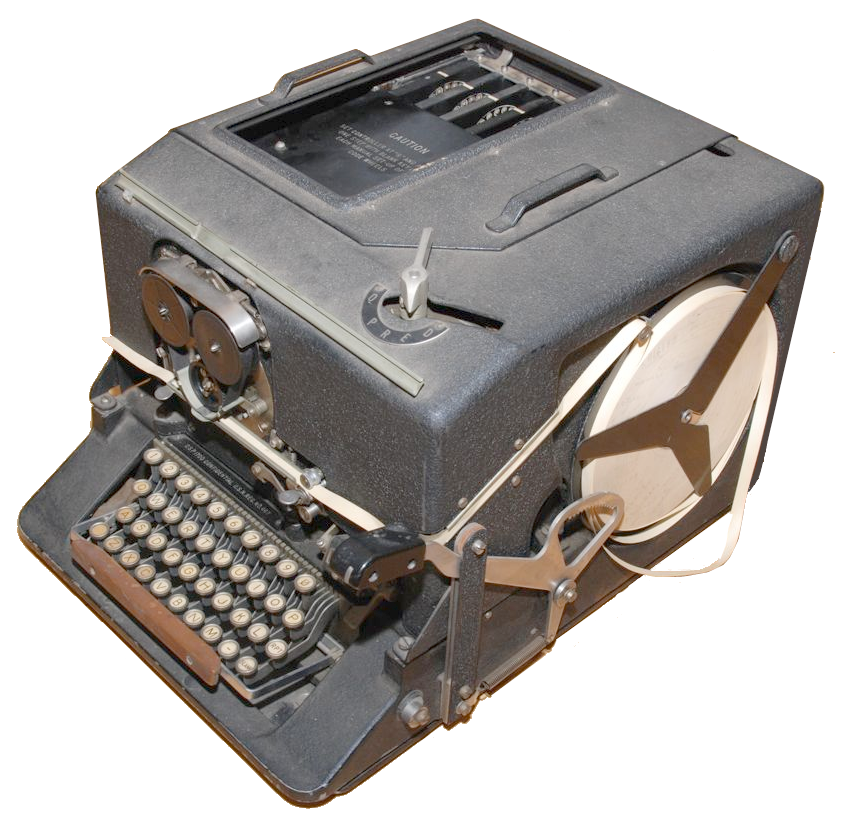
\includegraphics[width=0.3\textwidth]{pictures/SIGABA.png} 
	\caption{The SIGABA}
	\end{figure}

\end{frame}
% ------------------------------------------------------------------------------------------------

\begin{frame}
      \frametitle{Plan}
    We choose to speak of the Navajo code talkers who are the best know
    and whose story is declassified since 1968. Moreover, according to 
    the NY times, the Navajo code is the only spoken military code never to have
    been deciphered.

    %https://www.nytimes.com/2014/06/06/us/chester-nez-dies-at-93-his-native-tongue-helped-to-win-a-war-of-words.html?\_r=0)

    Plan
    \begin{itemize}
	\item relation of Navajo and the US in the late  of the 19th century;
	\item how Navajo code talkers have been recruited;
	\item study of the Navajo code. 
    \end{itemize}
\end{frame}
% ------------------------------------------------------------------------------------------------

\begin{frame}
\section{Navajos and US in the late of the 19th century}
    \begin{itemize}
    \item The long walk
    \item Boarding schools 
    \end{itemize}
\end{frame}

\subsection{The Long Walk (1984)}
\begin{frame}
    \frametitle{The long walk}
    According to the website navajocodetalkers.org, Navajo long walk is considered as one of the 
    most important parts of Navajo history. 

    \begin{itemize}
	\item  deportation of approximatively 8000 Navajo people by the
	       government of the United States of America
	\item forced trek over 480km into the Bosque Redondo camp.
	\item Many began the walk exhausted and malnourished
    \end{itemize}
     
    They were never informed as to: 

    \begin{itemize} 
	\item where they were going; 
	\item why they were being relocated; 
	\item and how long it would take to get there. 
    \end{itemize}

    The journey lasted 18 days, nearly 200 Navajos died of exposure 
    to elements and starvation. 

\end{frame}
% ------------------------------------------------------------------------------------------------

\subsection{Boarding schools }
\begin{frame}
    \frametitle{Boarding schools}

     At begin of the 20th century, many American Indian children were in 
     church-operated boarding schools.

    Children were forced to
    \begin{itemize}
	\item speak in english and not in their native language
	\item cut their hair and give up their traditional clothing;
	\item give up their meaningful Native names and take English ones; 
	\item replace their traditional religious practices by Christianity. 
	They were taught that their cultures were inferior. 
    \end{itemize}
\end{frame}
% ------------------------------------------------------------------------------------------------

\begin{frame}
    \frametitle{Boarding schools}
    %Many Code Talkers attended boarding schools. 
    %Schools were run like military organizations and this
    %made it easier for them to adapt to life in the American military.
    %As adults, they found it puzzling that the same government that had tried to take
    %away their languages in schools later gave them a critical role speaking their
    %languages in military service.

    \begin{quote}
	They tell us not to speak in Navajo language. You�re going to school.
	You�re supposed to only speak English. And it was true. They did practice
	that and we got punished if you was caught speaking Navajo.
	
	John Brown, Jr., Navajo Code Talker, National Museum of the American Indian interview,
	2004
    \end{quote}
	
\end{frame}
% ------------------------------------------------------------------------------------------------

\begin{frame}
\section{Navajos as code talkers: how they have been recruited}
    \begin{itemize}
	\item Preliminary: the code talkers during the WWI
	\item Pacific war and the idea of Philip Johnston
	\item The demonstration
    \end{itemize}
\end{frame}
% ------------------------------------------------------------------------------------------------

\begin{frame}
    \frametitle{Preliminary: the code talkers during the WWI}
    \begin{itemize}
    \item First use of native American code talker : Cherokee. 
    \end{itemize}
	    
    During Second Battle of the Somme in September 1918. 

    Germans tapped into telephone lines of American, break their codes,
    and captured runners send out to deliver messages directly. So, they have some
    tactical plans of enemies in their hands.

    Captain Lawrence of US Army eared two Choctaw talking together in their own
    language. 
	
    This give him the idea to use them to build a code with 20 terms
    and transmit secret tactical messages in their native language.

    They helped to win during the Meuse-Argonne Offensive.
\end{frame}  
% ------------------------------------------------------------------------------------------------


\begin{frame}
    \frametitle{Pacific war and the idea of Philip Johnston}

   % \begin{itemize} 
%	\item December 7 1941: Attack on Pearl Harbor
%	\item Pacific war: 7 December 1941 - 2 September 1945		
%    \end{itemize}

    % ![Philip Johnston](pictures/Jonhston.jpg)
     

    Philip Jonhston
	\begin{figure}
	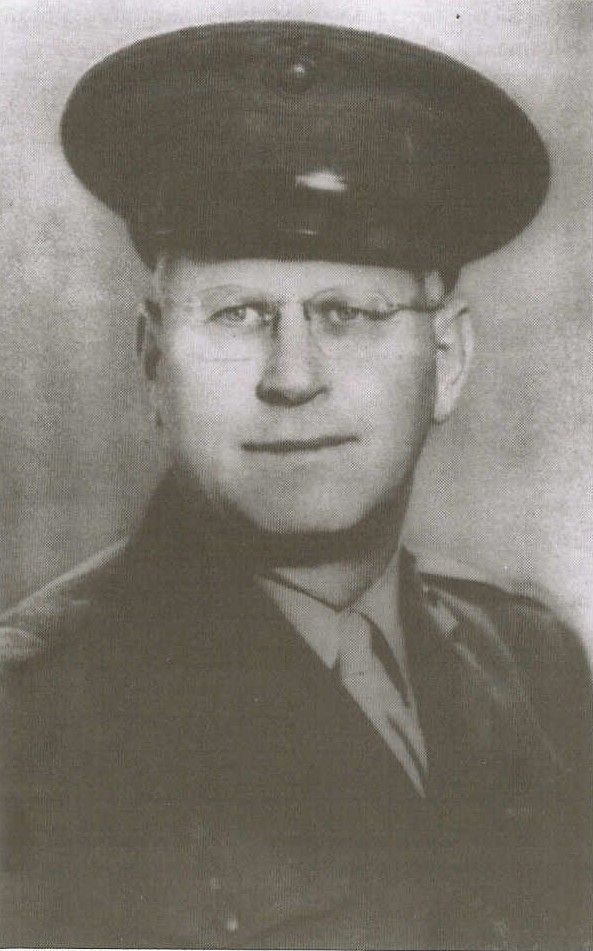
\includegraphics[width=0.15\textwidth]{pictures/Jonhston.jpg} 
	\end{figure}

    
    
    \begin{itemize}
    \item at 9 years old, he was  asker to  serve as an interpreter for a Navajo
    delegation. 
    \item 1942: he proposed to the Marine Corps that Navajos and
    other tribes could be recruit as code talkers.	
    \end{itemize}
TheThe major general Clayton
    Barney Vogel accepted to give this idea a try.
    
\end{frame}
% ------------------------------------------------------------------------------------------------

\begin{frame}
    \frametitle{The demonstration}

    Johnston recruited four bilingual Navajos and, on February 28,
    they go to Camp Elliott for a demonstration. 

    \begin{itemize}
    \item Two of the Navajos translated in Navajo typical military field orders
          and sent it by radio to their companions;
    \item The companions translated the message in English.
    \end{itemize}

    Example, 

    \begin{quote}
    "Enemy expected to make tank and dive bomber attack at dawn." 
    \end{quote}
    
    \begin{quote}
    "Enemy tank dive bomber expected to attack this morning." 
    \end{quote}
\end{frame}
% ------------------------------------------------------------------------------------------------

    
\begin{frame}
    Translation was done in 20 second instead of the 30 minutes needed by machines at that time.

    \begin{itemize}
    \item After this demonstration, Clayton wrote a
    letter to the commandant of the Marine Corps recommending the Navajo code
    talkers;
    \item May 1942: 29 Navajos recruit task develop a Navajo code.
    Altogether, between 375 to 420 Navajos participate to the program. 
    \end{itemize}

    %![the letter](pictures/letter.jpg)
\end{frame}
% ------------------------------------------------------------------------------------------------

\begin{frame}
\begin{center}
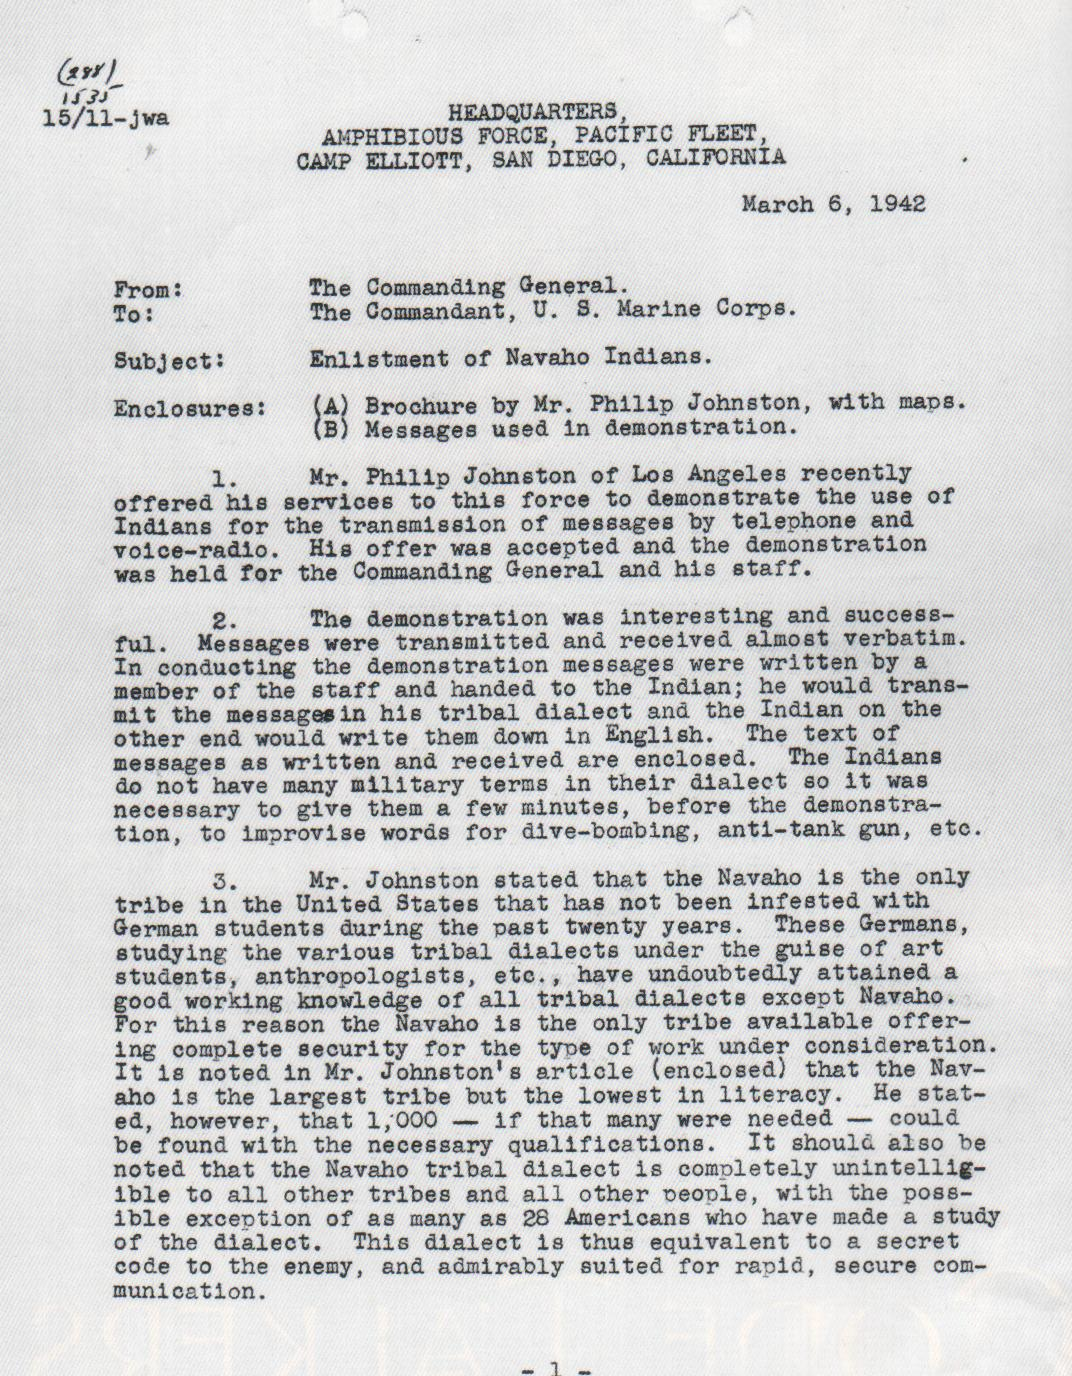
\includegraphics[width=0.5\textwidth]{pictures/letter.jpg} \newline
\tiny{https://www.archives.gov/files/education/lessons/code-talkers/images/letter-01.jpg}
\end{center}

\end{frame}
% ------------------------------------------------------------------------------------------------

\begin{frame}
\section{Navajo and Navajo code}
    \begin{itemize}
	\item Why the Navajo language was a good choice
	\item How the code works
	\item Some flaws of the code
	\item Some evolutions of the code
    \end{itemize}
\end{frame}
% ------------------------------------------------------------------------------------------------

\begin{frame}
	\frametitle{Why the Navajo language was a good choice?}
    	\begin{itemize}
	\item The largest population of Native American so the possibility to recruit and
	  from enough code talkers;
	\item It remained mostly "unwritten".
	\item Except the Navajos, only a handful of American experts were able to speak 
	  langage. 	
 	\item Navajo has a complex grammar, different from German and Japanese 
	\item faster than any machine at this time.
	\item It's difficult to to distinguish the sounds for uninitiated Navajo Speakers;
	\item Imposture aren't easy to make: it require to speak Navajo with a good accent.
    \end{itemize}
    PUT HERE a sample of the Navajo language. 
\end{frame}
% ------------------------------------------------------------------------------------------------

\begin{frame}
    \frametitle{How it works}
    Because of a lack of military terms in the Navajo language, there was the need
    for a code which consist in two different parts:
    \begin{itemize}
	\item Dictionary for common military words;    
    \end{itemize}

\begin{center}
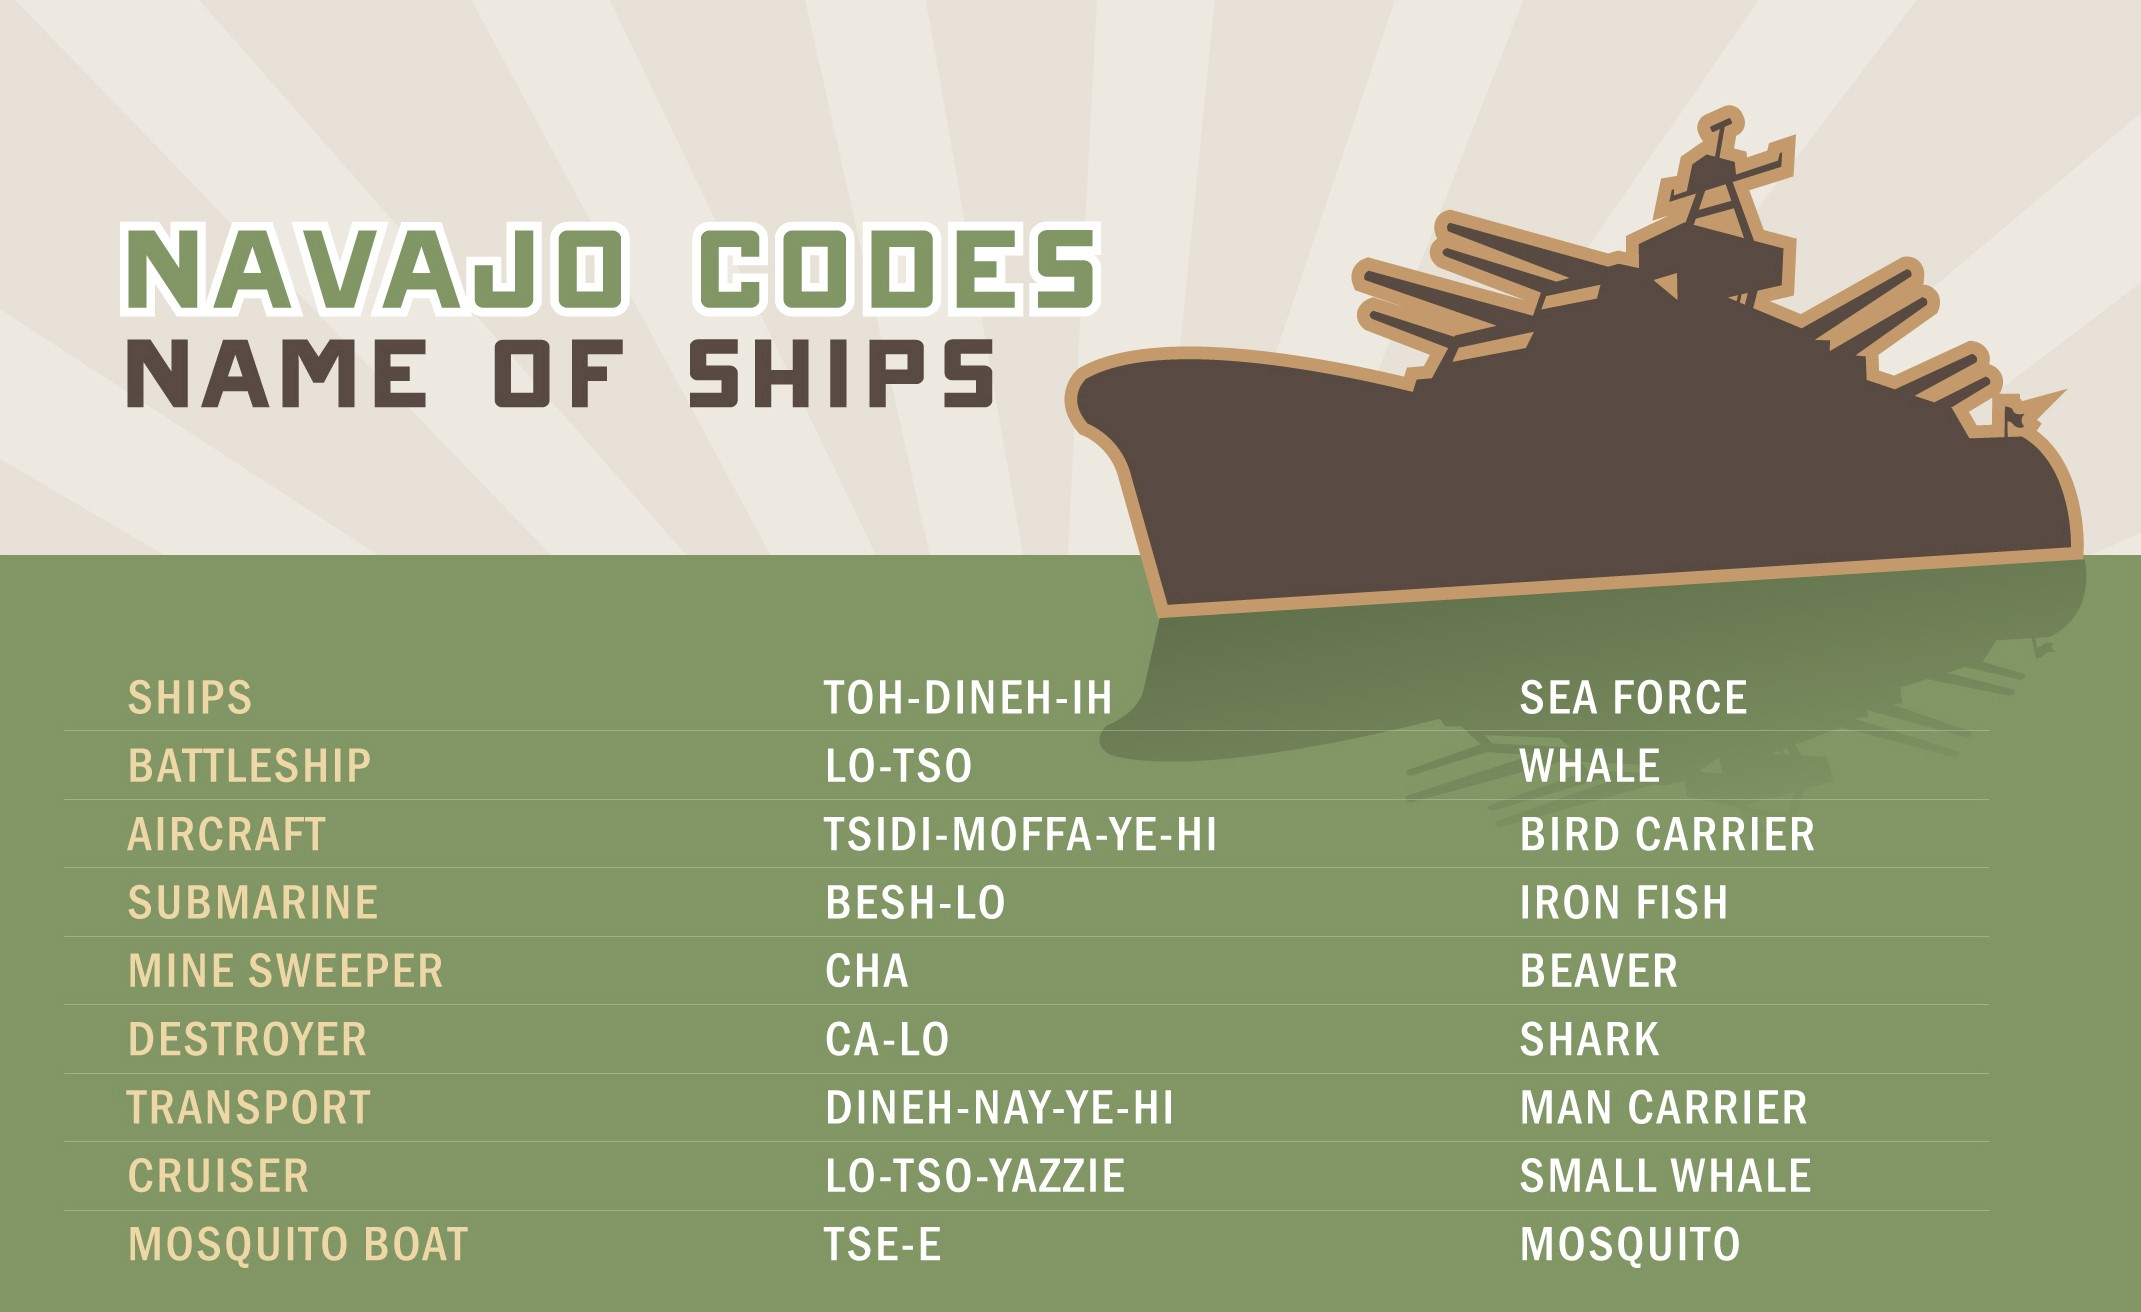
\includegraphics[width=0.7\textwidth]{pictures/ships.jpg} \newline
    \tiny{https://www.cia.gov/news-information/featured-story-archive/2008-featured-story-archive/navajo-code-talkers/}
\end{center}
\end{frame}
% ------------------------------------------------------------------------------------------------

\begin{frame}
    \frametitle{How it works}

    \begin{itemize}
    \item A phonetic alphabet table
    \end{itemize}

\begin{center}
    \begin{figure}[H]
\begin{tabular}{c|c|c}
\hline
A & WOL-LA-CHEE & Ant \\
\hline
B & NA-HASH-CHID & Badger \\
\hline
C & MOASI & Cat \\
\hline
D & CHINDI & Devil \\
\hline
E & AH-JAH & Ear \\
\hline
F & MA-E & Fox \\
\hline
\end{tabular}
	\caption{correspondance for some letters}
\end{figure}
	\tiny
	{https://www.cia.gov/news-information/featured-story-archive/2008-featured-story-archive/navajo-code-talkers/ }
\end{center}

%	      eagles, hawks, and all those domestic animals. Why don�t we use those names
%	      of different animals�from A to Z. So A, we took a red ant that we live with
%	      all the time. B we took a bear, Yogi the Bear, C a Cat, D a Dog, E an Elk, F,
%	      Fox, G, a goat and so on down the line.�Chester Nez, Navajo Code Talker,
%	      National Museum of the American Indian interview, 2004

\end{frame}
% ------------------------------------------------------------------------------------------------

\begin{frame}
    \frametitle{How it works}
	      \begin{itemize}
              \item Navajo Code Talkers memorized 17 pages of code during their training.
	      \end{itemize}
	      
	      A code talker answered one of his officers who had asked
	      why Navajos were able to memorize the complex code so quickly: 
	      
	      \begin{quote}
	      For us, everything is memory, it is part of our heritage. We have no written language.
	      Our songs, our prayers, our stories, they are all handed down from grandfather
	      to father to children and we listen, we hear, we learn to remember
	      everything. It is part of our training.\par
		  
	      (Power of a Navajo: Carl Gorman, the
	      Man and His Life, by Henry and Georgia Greenberg,1996) 
	      \end{quote}
\end{frame}
% ------------------------------------------------------------------------------------------------

\begin{frame}
    \frametitle{Some flaws of the code}
    \begin{itemize}
	\item non uniqueness of the translations on a message;
	\item Navajos trained at different times and place used sometimes 
	diff�rents words for specific military vocabulary, the solution;
	was to frequently "exchange" Navajos from one division into another;
	\item There was not enough code talkers and some battalions remained without 
	the capacity to decrypt or encrypt messages;
	\item Kerckhoffs's principles aren't observed.
    \end{itemize}


	      
\end{frame}
% ------------------------------------------------------------------------------------------------

\begin{frame}
    \frametitle{Evolution of the code}
    \begin{itemize}
	\item The original 211 vocabulary terms has been progressively 
	expanded to 411.
	\item  Multiple words to spell one letter.
    \end{itemize}

    \begin{center}
    \begin{figure}
    \begin{tabular}{c|c|c}
	\hline
	A & WOL-LA-CHEE & Ant \\
	\hline
	A & BE-LA-SANA & Apple \\
	\hline
	A & TSE-NILL & Axe\\
	\hline
    \end{tabular}
	\caption{multiple correspondances for one letter}
    \end{figure}
	\tiny
	{https://www.cia.gov/news-information/featured-story-archive/2008-featured-story-archive/navajo-code-talkers/ }
    \end{center}
\end{frame}
% ------------------------------------------------------------------------------------------------

\begin{frame}
\section{Conclusion:}
\end{frame}
% ------------------------------------------------------------------------------------------------
 
\begin{frame}
\frametitle{Declassification and recognition of code talkers after the war}
The program has been classified until 1968.

 
\begin{itemize}
	\item In 2000, the US Congree passed legislation to honor the Navajo Code Talkers
	  and give them special gold and silved congressional medals.
	\item In 2008, the Code talkers recognition act was signed into law by president
	  George W. Bush, which recognizes every other native american code talker who served
	  in the United States military durring WWI or WWII 
      
      \item In 2017, during a White House event specifically intended to honor the Navajo 
	 code talkers, Trump used the nickname "Pocahontas" to deride Elizabeth 
	 Warren, a political opponent.
    \end{itemize}
\end{frame}
% ------------------------------------------------------------------------------------------------

\begin{frame}
    \frametitle{Sources used}
    \begin{itemize}
    \item  https://www.archives.gov/education/lessons/code-talkers
    \item https://navajocodetalkers.org/navajo-long-walk/
    \end{itemize}
\end{frame}
% ------------------------------------------------------------------------------------------------

\end{document}
